\chapter{Fundamentals} % Main chapter title
\label{chap:fund}

% Hier muss alles rein was benötigt wird um die Arbeit zu verstehen.
%   Man kann ja sicherlich grundlegendes Verständis von Recherstrukturen und Organisation vorraussetzten
%   Was also sollte definitiv nochmal erklärt werden?
%
%   - Virtual Memory -> Und vor allem die Kosten, das ist ja auch irgendwo der Aufhänger
%           Der Satz, "tlb is on the critical path of everything really" sollte irgendwann mal kommen
%   - Motivation für vm
%   - Organisationsstrukturen auch im vergleich -> Fazit: Page Tables sind überall und werden tiefer -> vor allem wegeb backwards compatiblity?
%   - Hardware Strukturen für VM - MMU, TLB
%   - Operating system and VM -> Implemented by OS but fixed structures given by MMU
%   -> Problem, fehlende flexibilität ->  A look at several ...
%   -> source: Architectural and operating system support for virtual memory
%   source: issues of implementation

% -------------------------------------------------------------------------------------------------
% A little bit of history?? -> [Denning VM '96] -> Altas
% -------------------------------------------------------------------------------------------------
Der erste Computer mit virtual memory war Atlas \cite{fotheringham1961dynamic}. Die Grundidee war den
Programmen die Illusion zu schaffen, dass sie einen sehr großen Addressraum für sich alleine haben.
Dieser virtuelle Addressraum war dabei größer als der physische HauptSpeicher selbst.
Damit wurde auch die Aufgabe den physischen Hauptspeicher zu verwalten komplett vom Program gelöst
an das betriebssystem gegeben. Dessen Aufgabe ist war es nun die Teile des virtuellen Speicherbereichs
in den physischen Speicherbereiches zu laden, die auch vom Program in Ausführung benötigt werden.
\cite{denning1970virtual}.
Dies erhöht die Flexibilität für Programme extram, da diese nun nicht nur Daten in ihrem ganzen
virtuellen Addressraum verteilen können, sondern auch größer sein können als der physikalische Speicher
(solang genug Hintegrundspeicher zur Verfügung steht)\todo{CITE}\todo{thrashing irgendwo erwähnen?}.

% -------------------------------------------------------------------------------------------------
%                                           VIRTUAL MEMORY
% -------------------------------------------------------------------------------------------------


\section{Virtual Memory}
\subsection{Motivation}
Virtual memory is used in almost every system, ranging from big data center machines to small embedded system.
Originally, it was developed by the designers of the Atlas Computer to automate the task of swaping data between
main and secondary memory \cite{denning1997before}.

This was necesarry as programs increased in size faster than main memory did; while single programs
still fit in memory, operating systems allowed running multiple programs at once, collectively exceeding
the available physical memory \cite{tanenbaumOS}.

Nowadays, virtual memory is the basis of a lot of memory system requirements such as address
space protection, isolation of processes, shared memory and more \cite{jacobSoftwaremanagedAddressTranslation1997}.
It is also completely transparent to the programmer and enables programms to use every available
address in its virtual address space\cite{jacob1998look}.\\

Peter Denning calls its wide spread adoption ''[..]one of the engineering triumphs of the computer
age.''\cite{denning1997before}.
\subsection{Memory System Requirements/Benefits?}
Inzwischen erfüllt Virtual Memory noch sehr viel mehr Aufgaben als das Tauschen von Seiten in
Haupt und Nebenspeicher zu automatisieren. Virtual Memory Systeme sind Grundlage für
viele weitere Aufgaben und Features des Betriebssystem\cite{jacobSoftwaremanagedAddressTranslation1997}:
\begin{itemize}
    \item Address Space Protection / Isolation / Security
    \item Shared Memory
    \item Large Address Spaces
    \item Fine Grained Protection
    \item Sparse Address Space
    \item Superpages
    \item Memory Mapped Files / IO \cite{tanenbaumOS}
    \item Flexibilität für den Programmieren: Komplette Freiheit der Nutzung des Addressraumes
\end{itemize}
Diese Eigenschaften setzen die meisten Leute die auf Applikationsebene Programmieren mehr oder
weniger als gegeben voraus und machen sich keine weiteren Gedanken darüber\todo{cite?}.
Durch das immer weiter Auseinanderdriften der CPU und Memory geschwindigkeiten und vor allem
durch das größer werden von Addressräumen (von 32 auf 64 bit!) \todo{cite} sind die Ansprüche an
das Virtual Memory system gewachsen und so mussten sich auch die Implementationen weiterentwickeln.

Im Folgenden werden die meistgenutzten VM systeme betrachtet.
% VM Properties and benefits: Was für Nutzen hat VM?
% Fazit: VM hat sehr nützliche Eigenschaften
% More: jacob1998virtualissues

% -------------------------------------------------------------------------------------------------
%                                IMPLEMENTATION OF VIRTUAL MEMORY
% -------------------------------------------------------------------------------------------------

% Wie können wir VM realisieren? -> Verschiedene Implementationen, Aber hier nicht auf die HW eingehen
%   [ A look at several...]
%   [ Issues of implementation]
\subsection{Implementation of Virtual Memory}
Every virtual memory system has to realize a mapping from virtual addresses of each processes
private, virtual address space to actual physical addresses that index data in main memory.
This section will provide an overview of the most commonly used virtual memory implementation.\\

\todo{page table splits, vpn -> tanenbaum}
% Naiver Page Table ansatz
Das einfachste wäre natürlich eine große Tabelle mit den virtuellen zu physischen mappings im
speicher zu halten. Bei einem 32 Bit virtuellen zu physischen mapping mit einer typischen Page Größe
von 4 KiBi ( $ 2^{12}$Byte), bräuchte man mindestens 20 Bit pro Page Table Entry (PTE), also mindestestens
\[ 20 * 2^{20} Bit = 20971520 / 8 Byte = 2.5 MiBi \]
pro Page Table. Und da jeder Prozess eine eigene Pagetable braucht um die Isolation und damit Grundlage
für Sicherheit im System zu gewährleisten kann das insgesamt recht teuer werden.
Normalerweise würde man die PTEs auch noch auf wordsize alignen um dann auch noch platz für weitere
Protection flags zu haben, was dann die größe der Pagetable noch auf 4 MiBi erhöhen würde.
Bei 64-bit Computern wäre dieser naiver ansatz völlig unpraktikabel.
\todo{tanenbaum -> numbers for paging}
\subsubsection{Hierarchical page tables}
\todo{Verschiedene andere namen -> aus den übersichtspapern [a look at several, issues of impl]}
Um die Speicherkosten der Verwaltung der Pages zu reduzieren benutzten die meisten \todo{cite?}
Virtual Memory Systeme eine Multi-Level Page Table, oder auch hierarchische Page Table genannt.
Diese ähnelt aber in ihrere Struktur weniger einer Tabelle sondern mehr einem Baum dessen Nodes tabellen
von PTEs sind.
Hier wird die Virtuelle Page nummer nochmal in mehrere Teile unterteilt. Jeder Teil der VPN
wird benutzt um eine kleiner Tabelle zu indizieren. Der indizierte PTE verweißt dann auf die
nächste kleinere Page Table, die dann entsprechend mit dem nächsten Teil der VPN indiziert wird.
Je nach implementierung können hier bis zu 5 weitere indirektionen anfallen.
Ein gängiges Schema wie es z.B. in der RISC-V ISA spezifiziert wird ist Sv39, dass insgesamt
3 Level pro Page Table Tree vorsieht\cite{riscvreader}. Dieses Schema is auch nochmal
in Figure \ref{fig:fund:pagetree} zu sehen.
\begin{figure*}[t]
    \centering
    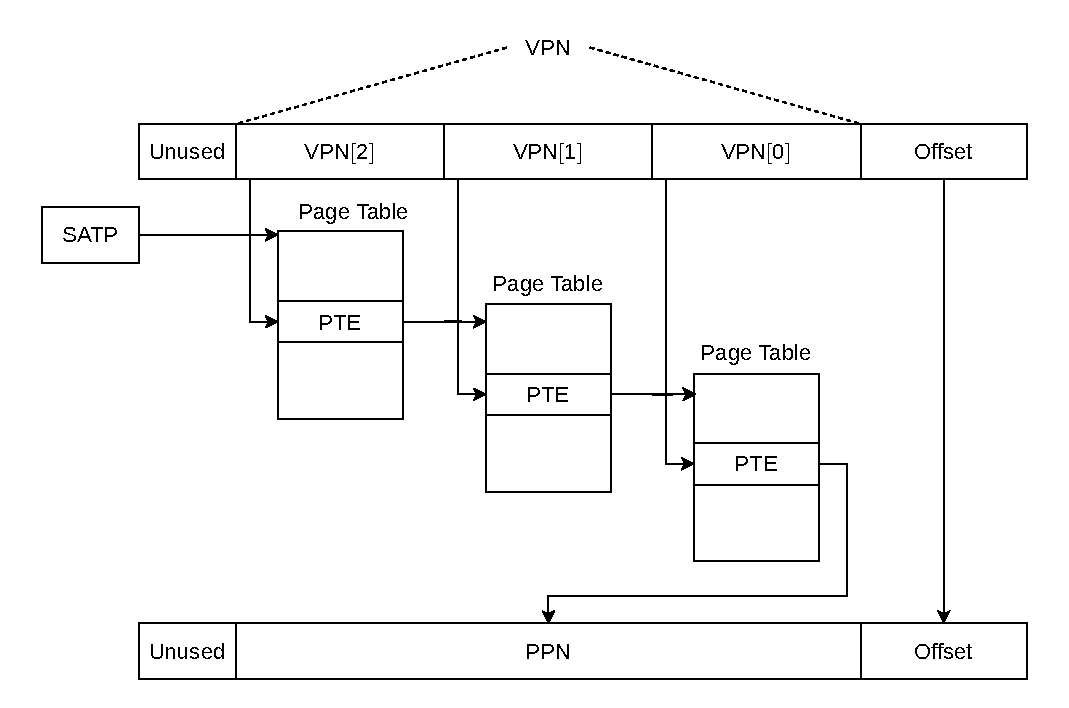
\includegraphics[scale=.8]{figures/VM-Tree.pdf}
    \caption[RISC-V Sv39 3-Level Page Tree]{Three-step page walk with a RISC-V Sv39 Page Table Tree:
        The value in the \texttt{satp} register is the base of the root page table; \texttt{VPN[2]}
        is the index into the root page table; the indexed \texttt{PTE} points to the next page table.
        This traversal continues until the bottom of the page table is reached. The last \texttt{PTE}
        contains the \texttt{PPN} of the physical address which can then be combined with the offset
        bits to make the full physical address}
    \label{fig:fund:pagetree}
\end{figure*}

% Fazit -> Viele Main Memory Zugriffe -> Teuer
Das traversieren der Page Table zum finden des Mappings benötigt pro Level eine weitere Memory reference\todo{cite}
und da das Ermitteln des Mappings auf dem kritischen Pfad jeder Memory-operation befindet,  sodass
es im schlimmsten fall, wenn alle caches missen, zu 5 memory accesses kommen muss (bei einem 5 -level
paging scheme) nur um das Mapping für einen Memory Zugriff zu finden.
% Lösung? Hashed!
\subsubsection{Inverted page tables}
Ein alternatives Paging schema geht von der anderen richtung an das ganze ran und stellt statt einen
Eintrag pro theoretischer virtueller Page einen PTE pro physischem Frame zur Verfügung.
Ein physisches Page Frame ist ein Page-aligneter platz im physischen speicher für eine Page.
Somit ergibt sich die anzahl der physischen Frames durch die Größe des Hauptspeichers geteilt
durch die Page-Größe \todo{Pages schon definiert? Auch die variable größe?}.
Vor allem für 64-bit Addressräume hat das den enormen Vorteil, dass nur so viele Seiten verwaltet
werden müssen die es auch tatsächlich physisch gibt.\\
Das Pagetable design hat noch den Vorteil, dass man im besten Fall deutlich weniger Hauptspeicherzugriffe
benötigt. In dem einfachen Design aus Figure \ref{fig:fund:inverted} kann der entsprechende
Page Table entry schon mit zwei Speicherlookups gefunden werden.

% worst case -> collision count only bound by page frame number
Da allerdings die Page Frame INdizies durch eine Hashfunktion aus der VPN berechnet werden, kann es zu
Hashkollisionen kommen. Da die Länge einer Kollisionskette nicht absehbar ist, ist die maximale
Anzahl der Speicherzugriffe um den richtigen PTE zu finden nur durch die maximale Anzahl der
Page Frames und damit durch die größe des Hauptspeichers beschränkt.

% hierachical -> fixed number of refs (but memory usage)
Hier haben die hierarchieschen multi-level page tables den entscheidenden Vorteil, dass sie immer
die feste Anzahl an Speicherzugriffen benötigen um den PTE zu ermitteln.
% Hash anchor to reduce the collision count
Typische Inverted page table designs haben meistens noch eine sogenannte Hash Anchor Table, die zwischen
dem Output der Hashfunktion und der Page Table liegt. Hat der Hash anchor doppelte größe
der Pagetable, lässt sich die durchschnittliche Collision Chain Length halbieren.
Allerdings wird nun mindestens eine Speicherreferenz in jedem Fall mehr gebraucht.
\cite{jacob1998virtualissues}

% Inverted Page Table figure
\begin{figure*}[t]
    \centering
    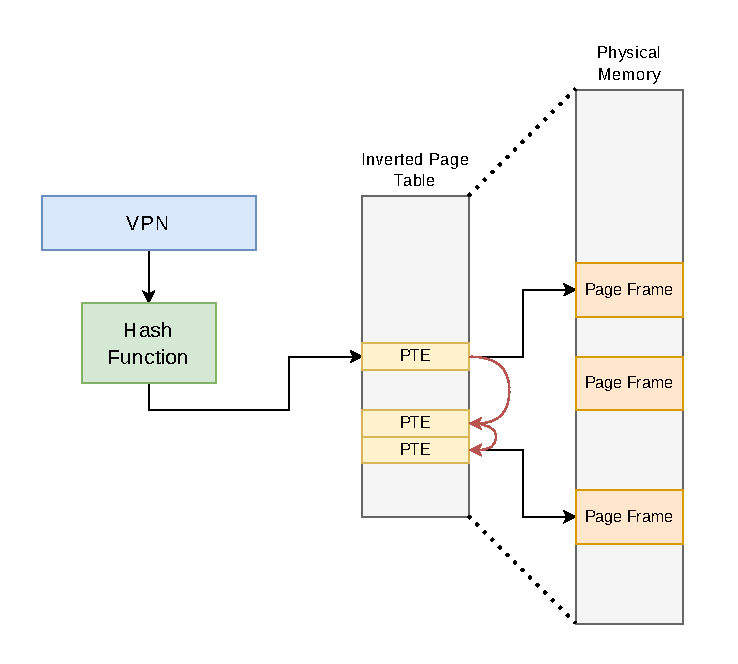
\includegraphics[scale=1]{figures/inverted_pt.pdf}
    \caption[Simple Inverted Page Table Design]{A inverted page table has an entry for every physical
        page frame, reducing memory accesses to a minimum of one. Collisions in the hash table (red arrows) can
        make the access much more expensive. }
    \label{fig:fund:inverted}
\end{figure*}
% Fazit-> Nachteile von Invertierten Page Tables [siehe auch hash dont cache!]
Inverted Page Tables reduzieren zwar die durchschnittliche Zugriffszeit auf die PTEs enorm, sie machen
es jedoch schwerer andere features wie superpages und memory sharing zu unterstützen.
Die Power Architecture unterstützt dies zum Beispiel durch einen zweistufigen übersetzungsprozess\cite{yaniv2016hash}.
% [hash dont cache] -> Hashed paging performs better


% [hash dont cache] -> superpages are harder

% [issues of impl] -> 

% [ A look at several] -> 

% -> Most commonly used in todays hardware -> Multi level page tables
Einen klaren sieger in der debatte hashed vs radix \todo{radix begriff noch einführen} gibt es nicht
und kommerzielle Hardware unterstützt verschiedenste designs die nicht standatisiert sich und z.t.
stark unterscheiden \cite{jacob1998look}.

Moderne INtel prozessoren unterstützen inzwischen radix designs mit einer tiefe von bis zu 5 ebenen,
die nach wie vor 4KB pages benutzten um Kompatibilität zu bewaren.

% Todo, aber größere pages erhöhen tlb reach usw
% Fazit -> Hauptproblem von VM sind teure Hauptspeicherzugriffe im kritischen Pfade von allen Memory Operations

\todo{discussion: Sind die aktuellen VM systeme (vor allem hierachical) noch Zeitgemäß oder nur noch altlast???}
% -------------------------------------------------------------------------------------------------
%                                  END SECTION - VM IMPLEMENTATION
% -------------------------------------------------------------------------------------------------



% -------------------------------------------------------------------------------------------------
%                                            VM HARDWARE
% -------------------------------------------------------------------------------------------------

\section{Memory Management Hardware}
Um die Umwandlung der virtuellen in physische Addressen weiter zu beschleuningen nutzen die meisten
modernen Rechner extra hardwarebausteine. Diese bestehen aus einem Hardware Page Table walker (MMU) und
einem Translation Cache, meistens Translation Lookaside Buffer (TLB) genannt\cite{jacobVirtualMemoryContemporary1998}.
% Frage: Besteht das MMU aus TLB + State Walker oder ist MMU der State Walker und TLB einfach extra?
% FIGURE Simple HW Architecture for VM Acceleration Hardware
\begin{figure*}[t]
    \centering
    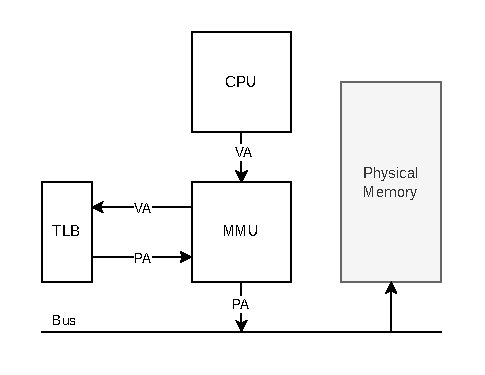
\includegraphics[scale=1.2]{figures/simple_mmu_arch.pdf}
    \caption[A simplified architecture of CPU, MMU and TLB]{A simplified architecture of CPU, MMU and TLB:
        User-level programs running on the \texttt{CPU} try to access main memory with virtual
        addresses; virtual addresses get transparently translated to physical addresses by the
        \texttt{MMU} by either looking up the address in the TLB or by performing a page table
        lookup with the hardware-supported page table design}
    \label{fig:fund:simplearch}
\end{figure*}
% End Figure

% Davor sollte der Page Table walk bekannt sein
\subsection{MMU}
Das Memory Management Unit (MMU) übernimmt die Aufgabe der addressübersetzung für den Computer.
Dabei steht es zwischen dem Prozessor, der hauptsächlich mit virtuellen Addressen arbeitet und dem
Memory Bus, der mit physischen Adressen zugegriffen wird. Greift der Prozessor auf eine gewisse
virtuelle addresse zu, so führt das MMU einen Page Table walk durch um die zu der virtuellen
Addresse passende physische addresse zu bestimmen. Währenddessen ist der Prozessor effektiv eingefrohren\cite{jacobVirtualMemoryContemporary1998}
\todo{more fine-grained citation? -> Probably not, these are only fundamentals, should however quote overarching works}
\subsection{TLB}
Weil es sehr teuer wäre bei jedem Lade oder Speicher Memory Zugriff einmal die Page Table in hardware zu durchgehen,
gibt es einen Cache für die Übersetzungen, den Translation Lookaside Buffer (TLB). Dieser Cache enthält
most recent Translations von virtueller zu physischer addresse.\\
Das MMU kann also erst mal in den TLB schauen, der parallelisiert und damit extrem schnell durchsucht
werden kann \cite{drepper2007every}.


% Gute quelle für alles hier : [jacob2010memory]
\cite{jacobVirtualMemoryContemporary1998}
% \subsection{A typical Page Table Walk}



% Fazit -> Es gibt hardware strukturen die VM beschleunigen können, die machen es auch schneller
%       ABER: Die machen die VM Software Systeme auch sehr viel rigider und unflexibler
% Kurze Diskussion -> Machen Hardware strukture das wirklich schneller? [ A look at ...]
% -------------------------------------------------------------------------------------------------

% -------------------------------------------------------------------------------------------------

\section{Sofware-based Virtual Memory System}
% VM in Software möglich mit ähnlicher Performance wie hw möglich -> Sollte ja mehr Flexibilität geben
%   [ A look at several...]
% \section{ Sofware VM Approaches}
% \section{ Liedtke GPTs}
% \subsection{More flexibilty}







\section{HW VM vs SW VM}
% related work will then come in to discuss approaches close to my approach
% With only software ptw process would have to context switch to the kernel -> Very expensive
% With an MMU the processor essentially just freezes until the memory operation has completed
% \subsection{HW-Dependent PTE Structure} -> inflexibility
Zwischen hardware und software managed translations gibt es einige Erwägungen die in betracht
gezogen werden sollten.

\paragraph{Feste Paging Structuren} Bei Hardware Managed Virtual Memory sind die structuren für
für die Page Tables und Page Table Entries fest von der Microarchitecture definiert.
Dadurch kann das Betriebssystem das Memory Management nicht auf seine zwecke und seinen Use case
zurecht schneiden und ist stuck mit dem fixen design.
Dieses erschwert auch die Portabilität von Systemsoftware, da es keinen Standard für diese
Memory Management Strukturen gibt.
Bei diesen gibt es auch keinerlei standartisierung obwohl es keine bedeutenden Performance unterschiede
in den Verschiedenen designs  gibt \cite{jacob1998look}.

\paragraph{Pipeline freezing / flushing} Bei einem TLB Miss \todo{schon definiert?} kommt es bei
einem hardware verwalteten TLB nur zu einem einfrieren der Pipeline (zumindest für die Instruktionen
die abhängig von dem Speicherzugriff sind). Bei einem software verwalteten TLB wird die Kontrolle
jedoch zurück an das Betriebssystem über eine Exception gegeben, die entsprechend vermerkt,
dass sich die benötigte Adresse nicht im TLB befindet (TLB Miss Exception).
Der Sprung zurück ins Betriebssystem sorgt für einen Context-Switch, es muss also der Zustand
des aktuellen Prozesses gespeichert werden. Dabei wird der Reorder buffer geflushed und die
pipeline massiv gestört. Durch den switch in den Kernel kann es langfristig auch noch zu weiteren
Data und Instruction misses kommen, da ja der Kerneleintritt sicherlich einige Cache lines die der
laufende Prozess benötigt hat überschrieben hat.

\paragraph{Embedded} Auch für embedded systems wird es interessanter virtual memory zu nutzen.
Diese würden sicherlich von flexibleren designs profitieren. Außerdem würde die ein Einsparen
an Chipgröße durch weglassen des MMUs auch die Kosten in der Produktion senken. \cite{jacob1998look}
\todo{weiß ja nicht}


% Conclusion of HW vs SW
\cite{jacob1998look} schließt in einer vergleichenden Studie verschiedener HW und SW memory designs,
dass wohl HW basierte Ansätze grundsätzlich performanter sind, aber das SW basierte designs durchaus
viable sind, wenn die caches groß genug sind um die Anzahl der Cache misses zu reduzieren.
Besonders bezüglich der flexibilität haben sw ansätze auch einen großen vorteil, da das VM system
vollständig durch das OS definiert werden kann.
% -------------------------------------------------------------------------------------------------

% -------------------------------------------------------------------------------------------------

% TODO Short discussion hw and sw vm -> common problem: Page Table Walks require in either case a 
% lot of memory references. These costs can be aleviated using caches, but will still cost [ cite a source abouts costs here]


% -------------------------------------------------------------------------------------------------

% -------------------------------------------------------------------------------------------------

% All approaches are based on a table.
% Überleitung zu meinem Thema -> Avoid all memory references and just have a simple (hash?) function that realizes VM
% [ a look at severeal ] -> conlsion